\chapter*{\FontH{\Huge Das Gespenst Jonathan}}
\addcontentsline{toc}{chapter}{Das Gespenst Jonathan}
\begin{mdframed}[style=mystyle]
\lettrine[lines=3]{\color{red}A}{m} besten stelle ich mich erst einmal selbst vor. Ich heisse Olivia Maibaum und bin neun Jahre alt. 

Vor drei Wochen habe ich zum ersten Mal in meinem Leben ein Gespenst gesehen und zwar ein richtiges! Einmal habe ich zwar schon einmal gedacht, dass ich eines sehe, das war dann aber doch nur die frisch gewaschene Jacke von Frau Maier, unserer Nachbarin. Der Wind hatte sie von der Leine gerissen und die ist mir dann entgegen geflogen gekommen, als ob da ein Gespenst durch die Luft schwebt. Hab ich mich damals erschrocken! Ich bin vor Schreck vom Fahrrad gestürzt und habe mir dabei die Hose zerrissen.  War das eine Aufregung und Mama wollte mir erst gar nicht glauben.

Aber das will ich hier gar nicht erzählen, die Geschichte vom richtigen Gespenst Jonathan ist viel interessanter.  Dass es Jonathan heisst, habe ich erst später erfahren. Aber ich will Euch mal die Geschichte von Anfang an erzählen.
\end{mdframed}

Mit einem lauten Krachen fällt die Rüstung von Ritter Odo von Gladez um. Die Weisse Frau von Burg Lauenstein kommt durch die Wand gleich hinter der Rüstung geflogen und sieht sich den Haufen alten Blechs auf dem Boden an.

\enquote{Jonathan!} ruft sie, \enquote{Komm sofort hierher!} Mit gesenktem Kopf kommt auch Jonathan durch die Wand. Jonathan ist der Sohn der Weissen Frau, die eigentlich Otilia Brigitta Walburg Peternella von Abendberg heisst. Aber alle nennen sie die Weisse Frau und das schon seit vierhundert Jahren. Sie ist nämlich ein Gespenst und die Mama von Jonathan, der natürlich auch eines ist. 
\afterpage{
    \begin{figure}
        \thispagestyle{empty}
        \centering
        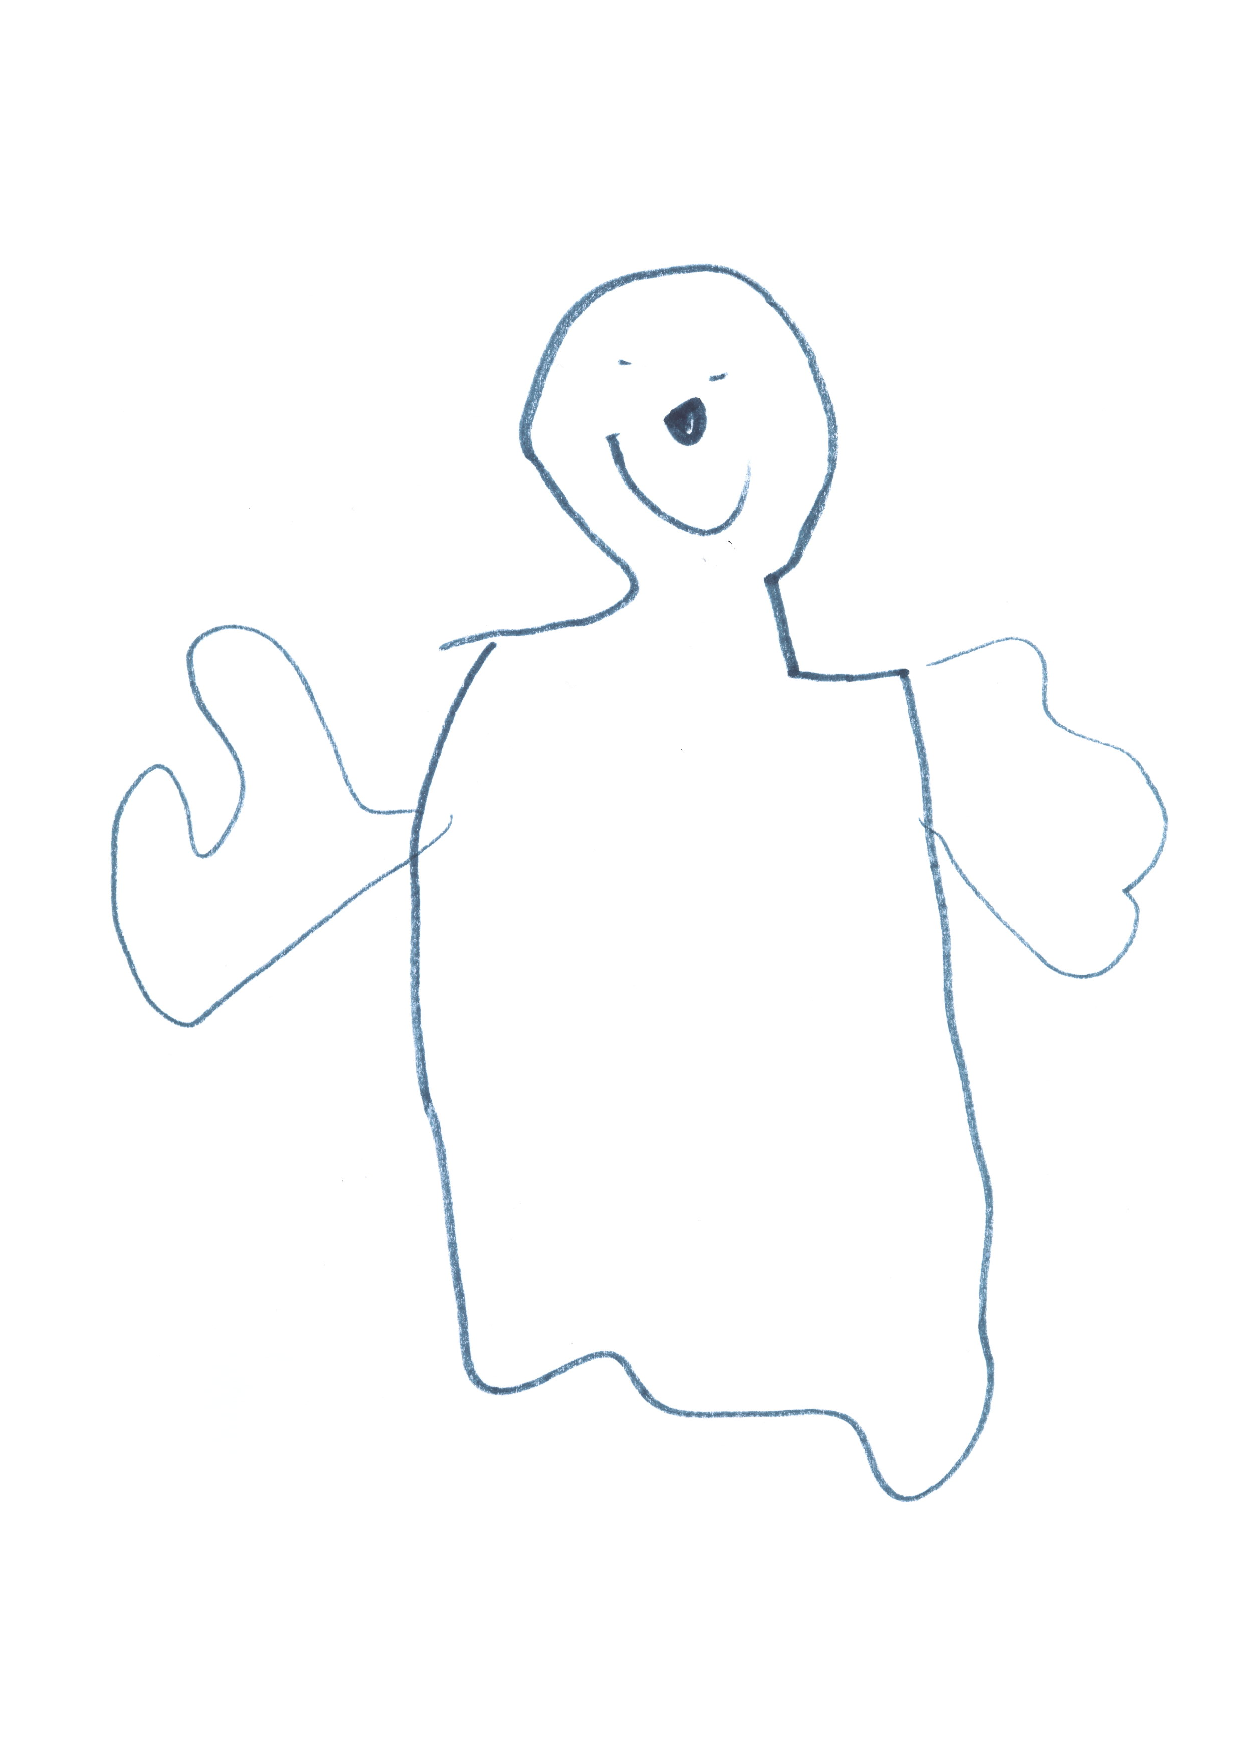
\includegraphics[width=\textwidth]{bilder/gespenst1.pdf}
    \end{figure}
    \clearpage
}

\enquote{Was soll ich nur mit Dir machen?} seufzt die Mama. Andauernd wirft Jonathan etwas um. Er passt einfach nicht auf, wenn er zu schnell durch die Wände geflogen kommt und nicht merkt, dass in dem Raum zum Beispiel eine Vase oder ein Kleiderständer steht. Gespenster können nämlich nur durch Wände fliegen, durch andere Sachen nicht. Und Jonathan war eben ein besonders schreckhaftes Gespenst. Immer wenn er glaubt, dass Menschen in der Nähe sind, nimmt er Reissaus und saust durch Burg Lauenstein, um sich zu verstecken. Besonders vor Kindern hat er furchtbare Angst. Die sind immer laut und frech und ärgern sich gegenseitig und ganz bestimmt auch ihn, glaubt er. 

\begin{mdframed}[style=mystyle]
Burg Lauenstein müsst ihr wissen, ist eine alte Burg, die hier und da schon auseinander fällt. Sie liegt auf einem Hügel, gleich bei unserem Dorf. Lange Zeit hat niemand dort gewohnt und alle Türen waren fest verschlossen. Seit ein paar Wochen kommen aber immer wieder Handwerker und Architekten und Bauleute und sehen sich da um. Burg Lauenstein soll nämlich renoviert werden. Es soll ein Museum werden, in dem man so alles Mögliche ansehen kann, zum Beispiel wie die Ritter früher so gelebt haben. Und mein Vater soll dort im Museum arbeiten. Er wird dann die Eintrittskarten verkaufen und auch sonst nach dem Rechten sehen, hat er mir erzählt.
\end{mdframed}

\enquote{Du weisst ganz genau, dass wir als Gespenster immer ganz leise sein müssen. Die Menschen haben schreckliche Angst vor uns, deswegen verstecken wir uns ja in alten Burgen und Schlössern. Aber wenn Du so einen Radau machst, ist es mit dem Versteck bald vorbei.} Jonathan ist beleidigt. Meckern, meckern, meckern. Seit Tagen hat Mama schlechte Laune. Wahrscheinlich hat das etwas mit den Menschen zu tun, die jeden Tag kommen und hier etwas umräumen und dort etwas ausmessen. Und die tragen alle alberne gelbe Helme. Das haben die Ritter schon wesentlich schicker ausgesehen, denkt Jonathan. 

Er beschliesst der Sache auf den Grund zu gehen und sich die Menschen einmal genauer anzusehen. Dazu braucht er aber eine gute Idee, die dürfen ihn keinesfalls sehen. Er schwebt ein bisschen durch die Burg und probiert es in einer Lampe, aber wenn die angemacht wird, wird es ihm bestimmt zu heiss. Vielleicht in einer Rüstung? Gerade als er probeweise aus dem Helm heraus guckt, muss er so kräftig niesen, dass die Rüstung laut klappert. Viel zu unsicher, entscheidet er. Dann eben in die alte Truhe. Durch die Löcher, die die Holzwürmer in die Truhe gefressen haben, kann er wenigstens alles hören. So wird es gemacht. Es wird auch schon langsam Tag und bestimmt kommen die Menschen bald. 


\begin{mdframed}[style=mystyle]
Gespenster müsst ihr wissen, sind ganz besondere Wesen. Eigentlich sind sie völlig harmlos, aber irgendwann ist einmal jemand auf die Idee gekommen, dass sie vielleicht gefährlich sein könnten, wenn sie ja immer durch alle Wände fliegen können. Und da haben die Menschen angefangen, sich vor ihnen zu fürchten und sie zu vertreiben. Eigentlich haben aber die Gespenster viel mehr Angst vor Menschen. Sie können Menschen eigentlich gar nichts tun, ausser sie einmal kräftig zu erschrecken, was sie hin und wieder auch gerne machen. Aber weil sie von den Menschen verfolgt werden, haben sie angefangen, nur noch in Häusern zu wohnen, in denen keine Menschen mehr wohnen. Und das sind eben meistens alte Burgen und Schlösser.

Solche Häuser haben nämlich auch noch einen weiteren grossen Vorteil. Wisst ihr nämlich was Gespenster essen? Staub! Der weisse Staub, der sich auf Dingen absetzt, wenn man nicht putzt. Und weil in verlassenen Burgen niemand putzt, ist es für Gespenster wie im Schlaraffenland. Ich glaube, weil sie nur Staub essen, sind sie auch so weiss.

Irgendwann wurden Burgen nicht mehr gebraucht, ausser um ein Restaurant oder ein Museum darin aufzumachen. Aber so viele brauchen wir ja davon auch nicht, die anderen hat man einfach nicht mehr repariert und sie sind zerfallen. Gespenster, die in einer solchen Burg leben, haben eigentlich nur eine Chance. Es muss jemand kommen und ihre Geschichte aufschreiben. Dann können die Gespenster für immer in der Geschichte weiter leben. Aber dafür müssen sie erst einmal jemanden finden, der das macht.
\end{mdframed}

Heute darf Olivia ihren Vater zur Burg begleiten. Die Bürgermeisterin wird da sein und noch ein paar andere Leute, die sie nicht kennt. Ihr Vater ist etwas aufgeregt, da heute entschieden wird, wie es mit Burg Lauenstein und damit mit seiner Arbeit weiter gehen wird. Wie immer schütteln sich alle Erwachsenen die Hände und tätscheln Olivias Kopf, bevor endlich die schwere Tür zur Burg aufgeschlossen wird und alle endlich hinein dürfen. Die Augen müssen sich erst an das dämmerige Licht gewöhnen. Draussen scheint die Sonne, aber hier kommt sie nicht wirklich rein.

Die Erwachsenen bleiben stehen und fangen an Dinge zu diskutieren, die Olivia nicht so genau versteht. 

\enquote{Herr Maibaum, ihre erste Aufgabe wird wohl sein, hier einmal richtig aufzuräumen und den ganzen Staub und Dreck zu entfernen. Dann kommen Frau Doktor Hampel und Herr Doktor Wagner von der Universität und gemeinsam werden Sie eine Liste all der Sachen erstellen, die es hier gibt.} hört Olivia die Bürgermeisterin zu Ihrem Vater sagen, dann ist es ihr schon zu langweilig und sie fängt an, sich selbst etwas umzusehen.

All die Rittersachen mag sie nicht, dass merkt sie schnell. Schwerter sind dafür da gewesen, andere umzubringen, die findet sie blöd. Und als sie die Rüstungen sieht, überlegt sie, ob es nicht schrecklich unbequem gewesen sein muss, so ein Ding anzuhaben. 

Eine Maus läuft direkt auf sie zu. Die scheint gar keine Angst zu haben. Olivia lacht und sagt:

\enquote{Du bist viel mutiger als die Ritter in ihren Blechrüstungen.} So mutig ist die Maus aber doch nicht und verschwindet im Dunkeln. Olivia versucht hinterher zu rennen, aber plötzlich fällt ihr Blick auf eine grosse, schwere Truhe. Ihre Augen glänzen. So eine hat sie schon einmal in ihrem Buch mit Piratengeschichten gesehen. Da war dann ein unglaublicher Schatz in der Truhe. Ob hier wohl auch einer drin ist? Sie versucht den schweren Deckel hoch zu heben, aber das klappt nicht. Viel zu schwer. 

Herr Wagner, der später ihrem Vater helfen soll, kann sofort erraten, was sie da macht. 

\enquote{Na, suchst Du Schätze?} will er wissen. Olivia fühlt sich ertappt und weiss nicht was sie sagen soll. Aber Herr Wagner lächelt, er scheint also nicht böse zu sein. Erwachsene sind ja schnell mal böse, wenn Kinder nicht genau das machen, was man ihnen gesagt hat. Olivia hat noch nicht ganz genau durchschaut, was man jetzt darf und was nicht und schon gar nicht, wenn es darum geht, Schätze in alten Burgen zu suchen.

\enquote{Warte, ich helfe Dir.} sagt er. Nett, denkt Olivia. Zusammen versuchen sie den Deckel zu heben, aber wieder klappt es nicht. Herr Wagner fängt an das Schloss zu untersuchen und runzelt die Stirn.

\enquote{Also verschlossen ist die Truhe nicht. Die klemmt, das kann bei so alten Truhen schon mal vorkommen.} Später kommen noch die Bürgermeisterin und andere Erwachsene hinzu und versuchen die Truhe zu öffnen, aber alle scheitern. Herr Wagner entscheidet, dass die Truhe als erstes aus der Burg geschafft werden soll und zwar direkt in die Werkstatt zu den Maibaums, damit er sie untersuchen kann.

\enquote{Vielleicht ist ja wirklich ein Schatz darin versteckt. Übermorgen komme ich und dann sehen wir uns das gemeinsam an.} sagt er und zwinkert Olivia zu. 

Was keiner der Anwesenden ahnt, ist das die Truhe keineswegs klemmt. Und ein Schatz befindet sich auch nicht darin, sondern das kleine und sehr verängstigte Gespenst Jonathan. Der weiss vor lauter Angst gar nicht was er machen soll und hält den Deckel so fest zu wie er kann. Als Herr Maibaum und Herr Wagner die Truhe unter Schnaufen und Prusten hoch heben und auf ein Auto verladen, wird er fast ohnmächtig vor Angst. Was werden die wohl mit ihm machen?

Beim Abendessen ist Vater Maibaum sehr Aufgeregt und erzählt seiner Frau in allen kleinen Details, was wer gesagt hat und wie wer dabei geguckt hat. Das ist schon an normalen Tagen furchtbar langweilig für Olivia, aber heute ganz besonders. Erstens ist sie dabei gewesen und weiss das alles schon und zweitens will sie doch unbedingt nochmals in die Werkstatt und sich die Truhe ansehen. 

Sie hat nämlich in Ihrem Piratenbuch nachgesehen. Da haben sie die Schatztruhe auch erst nicht auf bekommen, es dann aber mit einer Eisenstange geschafft. Wie genau weiss Olivia auch nicht, aber sie will es unbedingt noch heute versuchen. Als sie endlich vom Tisch aufstehen darf rennt sie sofort in die Werkstatt. Sie nimmt ein langes Rohr, das in der Werkstatt an der Wand steht und nähert sich der Truhe.

Das ist genau der Augenblick, als Jonathan es nicht mehr aushält und den Deckel vorsichtig öffnet, um mal einen Blick ins freie zu werfen. Er blickt durch den sich öffnenden Spalt und sieht wie ausgerechnet ein Kind, eines dieser gefährlichen Schreihälse, mit einer Stange bewaffnet auf ihn zu kommt. Das ist zu viel für ihn. Er schreit wie er noch nie im Leben geschrieben hat.

\begin{mdframed}[style=mystyle]
  Ihr könnt euch vorstellen, dass es mir nicht viel anders erging als Jonathan. Als sich plötzlich der Deckel wie von alleine geöffnet hat und ein echtes Gespenst zu sehen war, das auch noch geschrien hat wie verrückt, habe ich vor Schreck die Stange fallen lassen. Das hat einen so lauten Knall gegeben, dass sofort Papa in die Werkstatt gestürzt gekommen ist, und wissen wollte, was los ist. Ohne meine Antwort abzuwarten hat er gleich geschimpft und gemeint, die Kiste dürfe ich nicht anfassen, die sei alt und \textit{wissenschaftlich wertvoll}, wie er das mit wichtiger Mine genannt hat. Da dürfe nichts kaputt gehen, nicht einmal ein kleiner Kratzer sei erlaubt. Dabei ist die Kiste doch uralt und schon von alleine ganz wurmstichig. 
  
Verstanden habe ich das nicht. Aber ich musste sofort ins Bett. Da habe ich es natürlich nicht ausgehalten. Als Mama und Papa endlich wie jeden Abend vor dem Fernseher eigeschlafen waren, bin ich sofort wieder in die Werkstatt geschlichen. Zweimal tief Luft holen musste ich schon. Immerhin war ja ein Gespenst in der Werkstatt. Ich habe all meinen Mut zusammen genommen und habe die Tür geöffnet. Jonathan sass zitternd in der Ecke, weswegen ich plötzlich keine Angst mehr hatte. 
\end{mdframed}

Olivia geht langsam auf das Gespenst zu. 

\enquote{Ich heisse Olivia und wer bist Du?} fragt sie. Jonathan bekommt erst kein Wort heraus, merkt aber auch schnell, dass das Mädchen wohl doch nicht so gefährlich ist, wie er erst dachte. Erst sagt er nur seinen Namen, aber dann sprudelt es aus ihm heraus. Dass er ein Gespenst sei, erzählt er -- als ob Olivia das noch nicht gemerkt hätte -- und dass er auf Burg Lauenstein wohne, seine Mutter die Weisse Frau sei, dass er Angst vor Kindern habe, aber eigentlich noch nie eines kennengelernt hat und noch so ein paar andere Dinge mehr. 

Olivia will natürlich auch gleich vieles wissen. Wie es ist, ein Gespenst zu sein und ob man als Gespenst zaubern kann. Kann man aber nicht. Naja, nicht wirklich zaubern, aber immerhin durch Wände gehen und das beeindruckt Olivia dann natürlich sehr. Stundenlang muss Jonathan durch die Werkstatt fliegen, durch die eine Wand raus durch die andere wieder rein, mal nur mit dem Kopf aus der Wand gucken und Grimassen schneiden. 

\enquote{Ich habe Hunger, willst Du auch was?} ruft Olivia und ohne eine Antwort abzuwarten saust sie in die Küche. Als sie am Wohnzimmer vorbei muss, zieht sie ihre Schuhe aus, damit es keinen Ton gibt und Mama und Papa munter werden. Mit Schokoriegeln in der Hand kommt sie zurück. Jonathan stutzt und meint, dass er als Gespenst natürlich nur alten Staub zum Essen mag und Schokoriegel ganz unter seiner Würde seien. Olivia ist zwar verblüfft, aber dann bleibt eben mehr für sie übrig. Und Staub gibt es in der Werkstatt mehr als zehn Gespenster in einem Jahr schaffen würden.

\enquote{Was haben eigentlich die vielen Leute heute bei uns in der Burg gemacht?} will Jonathan schmatzend wissen.

\enquote{Die haben sich angesehen, wie die Burg neu umgebaut werden soll. In ein Museum. Und mein Vater hilft auch mit und muss als erstes putzen. Schon in einer Woche geht es los.} weiss Olivia. Jonathan muss sich vor Schreck fast verschlucken.

\enquote{Aber dann haben wir ja gar nichts mehr zum Essen. Und wo sollen wir dann wohnen?} ruft er aufgeregt. \enquote{Dass muss ich sofort Mama erzählen.} und schon fliegt er los.

\enquote{Aber komm mich doch mal wieder besuchen!} kann Olivia ihm gerade noch hinterher rufen.

Schon am nächsten Tag kommt Jonathan zurück. Und mit ihm seine Mutter, die Weisse Frau. Es war schon dunkel und Olivia wollte sich gerade hinlegen, als es am Fenster klopft. Sie dachte sich zwar schon, wer das sein könnte, aber zur Sicheherheit nimmt sie ihren Teddy als Beschützer unter dem Arm mit. Sie bekommt dann doch einen Schrecken, als sie die Weisse Frau sieht. So ein ausgewachsenes Gespenst ist dann schon noch etwas anderes, als ein Kindergespenst. Olivia muss alles nochmals genau erzählen, was sie auf der Burg mitbekommen hat, als die Bürgermeisterin geredet hat.

Die Weisse Frau hört sich das alles an und muss hier und da nochmals nachfragen und sagt dann: 

\enquote{Da hilft alles nichts.} und streichelt dabei Jonathan über den Kopf, \enquote{Wir müssen umziehen.} Aber wohin? Keiner der Drei kennt eine leer stehende Burg. Olivia schaltet den Computer an und sucht im Internet.

\enquote{Nein, nichts.} sagt sie. Die einzige leere Burg, die sie finden kann, ist eine Ruine, aber die ist schon sehr zerfallen. Da stehen nur noch ein paar Mauerreste. Alle seufzen. Aber die Weisse Frau ist schon ein altes Gespenst und weiss einen Rat.


\begin{mdframed}[style=mystyle]
Und der Rat der Weissen Frau war, dass auch sie beide das machen müssen, was schon so viele Gespenster vor ihnen getan haben. Sie müssen nicht in eine andere Burg umziehen, sondern zu einer Geschichte werden. Über die weisse Frau gibt es schon viele Geschichten. Aber über Jonathan bisher noch keine einzige. Und deswegen bin ich von den beiden gebeten worden, die Geschichte aufzuschreiben, wie ich Jonathan kennen gelernt habe. Und das habe ich getan. Jonathan wohnt jetzt in dieser Geschichte, die ich euch gerade erzählt habe. 

Aber Vorsicht! Jeden, der die Geschichte hört, kommt Jonathan mindestens einmal besuchen. Er ist aber immer noch sehr ängstlich. Er versteckt sich dann irgendwo bei euch. Und wenn ihr es schon bald mal irgendwo klappern hört und ihr wisst nicht warum, dann war das bestimmt Jonathan. Und wenn mal ein Spielzeug von euch fehlt, dürft ihr auch nicht böse sein. Das hat sich dann Jonathan geborgt. Immer in derselben Geschichte zu wohnen, ist ja auch etwas langweilig. Aber er hat mir ganz fest versprochen, dass er euch euer Spielzeug immer schon bald zurückbringt. Aber seid so nett und putzt nicht immer so fest! Wenn Jonathan kommt, freut er sich immer, hier und da mal ein bisschen Staub naschen zu können. \hfill {\color{red}\decofourleft}
\end{mdframed}

